\documentclass[11pt,a4paper]{article}
\usepackage[utf8]{inputenc}
\usepackage[T1]{fontenc}
\usepackage[italian,english]{babel}
\usepackage[a4paper,margin=2.2cm]{geometry}
\usepackage{lmodern}
\usepackage{microtype}
\usepackage{xcolor}
\usepackage{graphicx}
\usepackage{float}
\usepackage{booktabs}
\usepackage{longtable}
\usepackage{tabularx}
\usepackage{array}
\usepackage{multirow}
\usepackage{amsmath,amssymb}
\usepackage{enumitem}
\usepackage{hyperref}
\usepackage{caption}
\usepackage{fancyhdr}
\usepackage{titlesec}
\usepackage[most]{tcolorbox}
\usepackage{lastpage}
\usepackage{setspace}
\usepackage{url}

\hypersetup{colorlinks=true,linkcolor=blue!50!black,citecolor=blue!50!black,urlcolor=blue!60!black,pdftitle={StarCraft II Match Outcome Prediction Paper Draft},pdfauthor={Jose}}

\definecolor{accent}{RGB}{28,56,110}
\definecolor{softblue}{RGB}{242,246,252}
\definecolor{softgray}{RGB}{246,246,246}
\definecolor{softwarn}{RGB}{255,249,235}
\definecolor{softgreen}{RGB}{240,248,242}
\definecolor{linegray}{RGB}{210,215,225}

\pagestyle{fancy}
\fancyhf{}
\fancyhead[L]{StarCraft II Match Outcome Prediction}
\fancyhead[R]{Jose}
\fancyfoot[C]{\thepage/\pageref{LastPage}}
\setlength{\headheight}{14pt}

\titleformat{\section}{\large\bfseries\color{accent}}{\thesection}{0.7em}{}
\titleformat{\subsection}{\normalsize\bfseries\color{accent}}{\thesubsection}{0.6em}{}
\titleformat{\subsubsection}{\normalsize\bfseries}{\thesubsubsection}{0.5em}{}
\setlist[itemize]{topsep=3pt,itemsep=2pt,leftmargin=1.3em}
\setlist[enumerate]{topsep=3pt,itemsep=2pt,leftmargin=1.5em}
\setstretch{1.08}
\setlength{\parindent}{0pt}
\setlength{\parskip}{0.55em}

\newtcolorbox{keybox}{colback=softblue,colframe=accent!55!black,boxrule=0.6pt,arc=2mm,left=2mm,right=2mm,top=1.4mm,bottom=1.4mm}
\newtcolorbox{pendingbox}{colback=softwarn,colframe=orange!55!black,boxrule=0.6pt,arc=2mm,left=2mm,right=2mm,top=1.4mm,bottom=1.4mm}
\newtcolorbox{resultbox}{colback=softgreen,colframe=green!40!black,boxrule=0.6pt,arc=2mm,left=2mm,right=2mm,top=1.4mm,bottom=1.4mm}

\begin{document}

\begin{titlepage}
\centering
\vspace*{2.2cm}
{\Large University of Genoa\par}
\vspace{0.4cm}
{\large Machine Learning Project\par}
\vspace{1.6cm}
{\Huge\bfseries StarCraft II Match Outcome Prediction\par}
\vspace{0.35cm}
{\Large From Replay Parsing to Group-Aware Experimental Validation\par}
\vspace{1.3cm}
\begin{tcolorbox}[width=0.88\textwidth,colback=softblue,colframe=accent,arc=2mm,boxrule=0.8pt]
This document is designed as the \textbf{main technical paper} of the project. It consolidates the current methodology, explains the logic of the pipeline, records the best results available from the frozen project material and documents the final audit-cleaned artifact package used for reproducibility review.
\end{tcolorbox}
\vfill
\begin{tabular}{rl}
Candidate: & Jose \\
Academic year: & 2025--2026 \\
Document version: & Revised freeze \\
Date: & March 2026 \\
\end{tabular}
\vfill
\end{titlepage}

\selectlanguage{english}

\section*{Abstract}
This project studies match outcome prediction in \emph{StarCraft II} using tabular snapshots extracted from real replay files rather than images or raw sequences. The technical objective is not only to train a classifier, but to build a complete and reproducible pipeline from replay parsing to inference. The dataset is generated from more than 24,000 competitive replays and sampled every 15 seconds after removing the first two minutes of game time. The work focuses on domain-aware feature engineering, group-aware evaluation to avoid replay leakage, and comparative analysis across Random Forest, XGBoost, and deep multilayer perceptrons.

A central methodological result is that naive row-based validation dramatically overestimates performance because adjacent snapshots from the same replay are highly correlated. Once the split is performed by \texttt{replay\_id}, the measured accuracy drops from the high-80\% range to roughly 61\%, which is far more realistic and scientifically meaningful. Current project materials now show that tree-based models form the strongest and most stable baseline on this tabular representation. The final GPU-trained MLP remains competitive but does not surpass the tree ensembles, and the strongest remaining advantage of XGBoost over Random Forest appears in probabilistic quality rather than in a large gain in raw accuracy. The paper also documents the remaining finalization steps, calibration evidence, and the roadmap for the last experimental cycle.

\tableofcontents
\newpage

\section{Introduction and Project Goal}
StarCraft II is a real-time strategy game with hidden information, long-horizon planning, macroeconomic management, and highly nonlinear interactions between army composition, technology, scouting, and timing. Predicting the winner from replay-derived tabular data is therefore an interesting machine learning problem for two reasons. First, it is a difficult supervised task with a meaningful target. Second, it forces the project to solve the much harder problem that comes \emph{before} training: how to convert a noisy temporal game trace into a structured dataset that preserves strategic signal.

The project goal is therefore twofold:
\begin{enumerate}
    \item build a replay-to-table pipeline that extracts strategically meaningful features at fixed time intervals;
    \item evaluate multiple supervised learning paradigms under a protocol that avoids information leakage between snapshots from the same match.
\end{enumerate}

\begin{keybox}
The classifier is only the last stage of the pipeline. The scientific value of the project depends equally on parser design, feature semantics, data cleaning, and validation protocol.
\end{keybox}

\section{Problem Formulation}
Let each replay generate a sequence of snapshots $x_t$ sampled at time $t$, with label $y \in \{0,1\}$ indicating whether Player 1 wins the match. The learning objective is to approximate
\[
    f(x_t) \approx P(y=1 \mid x_t)
\]
using a tabular representation of the game state. This framing has an immediate limitation: the model does not observe the full spatial or sequential structure of the game. Instead, it only sees the information that the parser chooses to encode. For this reason, the feature space must capture not only absolute state variables, but also relationships between the two players and local temporal momentum.

\section{Pipeline Overview}
The project pipeline can be summarized as follows:
\[
\begin{aligned}
&\text{Replay corpus} \rightarrow \text{SC2 parser / bridge} \rightarrow \text{snapshot dataset} \\
&\rightarrow \text{group-aware split} \rightarrow \text{model selection} \rightarrow \text{final evaluation}
\end{aligned}
\]

In practical terms, the project contains three tightly coupled layers:
\begin{itemize}
    \item \textbf{Replay ingestion}: reading \texttt{.SC2Replay} files and recovering player-level state at multiple times;
    \item \textbf{Feature engineering}: compressing military, economic, scouting, and compositional information into a fixed-width row;
    \item \textbf{Learning and validation}: comparing model families under a replay-aware evaluation protocol.
\end{itemize}

\section{Data Acquisition and Dataset Construction}
\subsection{Replay source and scale}
The broader project material references roughly \textbf{24,057} raw competitive or high-level replays, while the frozen \textbf{V3.1 fixed} benchmark retained \textbf{23,241} usable replays and \textbf{892,047} snapshots after the final filtering and parser-stability corrections. The extraction pipeline uses \texttt{sc2reader} for replay parsing and \texttt{joblib} for parallel execution. A key engineering point is that replay parsing is heavy enough that preprocessing itself becomes a relevant computational stage.

\subsection{Sampling policy}
Snapshots are extracted every \textbf{15 seconds}. Extremely short or atypically long games are removed, with the current filtering policy centered on durations between \textbf{180 s} and \textbf{1800 s}. In addition, the first \textbf{120 seconds} are removed from the learning problem because the opening phase is comparatively deterministic and contributes less discriminative variance.

\subsection{Why the first 120 seconds are removed}
The early game in StarCraft II often follows race-specific build order routines with low observable divergence in the aggregate statistics used here. Removing the earliest phase acts as a denoising step: it reduces the proportion of nearly identical low-information states and lets the models focus on strategic separation that emerges after the opening.

\subsection{Dataset identity structure}
Each row is associated with at least:
\begin{itemize}
    \item a \texttt{replay\_id},
    \item a snapshot timestamp \texttt{time\_sec},
    \item a binary label \texttt{p1\_wins}.
\end{itemize}
This identity information is not just metadata. It is essential for correct validation because all snapshots belonging to the same replay are statistically dependent.

\section{Feature Engineering Logic}
\subsection{Feature families}
The current project design includes four main semantic families:
\begin{enumerate}
    \item \textbf{Military power and army state}
    \item \textbf{Economic efficiency and production balance}
    \item \textbf{Scouting and informational behavior}
    \item \textbf{Temporal dynamics and momentum}
\end{enumerate}

The earlier presentation material reports around \textbf{30 columns} in the baseline parser actually used for the first experimental cycle, with \textbf{27 model features} after removing metadata and target. Newer parser branches already expose a richer feature space, including explicit counter-advantage and longer-horizon momentum features. This is important: the experimental results currently available mostly correspond to the earlier compact feature set, while the codebase is already evolving toward a second-generation dataset.

\subsection{Combat score}
A central domain-engineered variable is the \texttt{combat score}. Instead of using only raw unit counts, the parser builds a weighted military strength estimate based on:
\begin{itemize}
    \item per-unit base power,
    \item number of alive units,
    \item matchup-dependent counter penalties,
    \item upgrade and technology multipliers.
\end{itemize}
In the earlier project material, this design was motivated as a simple approximation to combat effectiveness beyond raw supply. In the newer parser branch, the combat logic is paired with an explicit counter-advantage computation and longer-horizon volatility features.

\subsection{Economic features}
Economic state is summarized through worker counts, income-related statistics, and especially \emph{Spending Quotient} (SQ), which tries to quantify how effectively a player converts resources and income into usable progress. In the prior project presentation, SQ is treated as a macroeconomic efficiency proxy and is one of the core inputs of all model families.

\subsection{Scouting and composition features}
The project also builds features that do not directly correspond to standard scoreboard metrics:
\begin{itemize}
    \item scouting score derived from camera movement and enemy-base attention,
    \item army entropy as a proxy for compositional diversity,
    \item number of unit types as a coarse signal of strategic flexibility.
\end{itemize}
These variables are particularly important because they encode behavior and composition rather than only scale.

\subsection{Dynamic features}
The first parser generation already introduced local deltas such as changes in workers, combat score, and SQ. The newer parser branch extends this idea with multi-horizon momentum terms (15 s, 60 s, 120 s), growth ratios, and rolling volatility estimates. This is one of the clearest directions for the next experimental phase because the outcome prediction task is inherently temporal even if the current models consume independent rows.

\section{Methodological Pivot: Leakage Control}
The most important scientific lesson of the project is that \textbf{row-level random splitting is invalid} for this dataset. Adjacent snapshots from the same replay share the same players, strategy arc, map context, and eventual label. If one snapshot goes to train and a nearby snapshot from the same match goes to test, the model is rewarded for memorizing replay-specific context rather than learning general strategic patterns.

For this reason, all serious evaluation must use replay-based grouping:
\begin{itemize}
    \item outer train/test split with \texttt{GroupShuffleSplit},
    \item inner cross-validation with \texttt{GroupKFold} whenever model selection is performed,
    \item no use of test data for early stopping or hyperparameter selection.
\end{itemize}

\begin{resultbox}
Current project materials report a sharp drop from roughly \textbf{87\%} apparent accuracy under row-based validation to about \textbf{61\%} under replay-aware validation. This is not a failure. It is the transition from an inflated estimate to a credible one.
\end{resultbox}

\section{Model Families and Expected Behavior}
\subsection{Random Forest}
Random Forest is a strong baseline for this dataset because the inputs are already engineered tabular variables with nonlinear thresholds and interactions. It does not require feature scaling, is robust to heterogeneous feature magnitudes, and can learn discrete rule-like partitions that fit many RTS situations.

\subsection{XGBoost}
XGBoost is attractive for the same reasons as Random Forest, but with sequential residual correction and stronger capacity to exploit subtle interactions. The current implementation uses GPU acceleration with histogram-based tree construction and early stopping on a dedicated validation split.

\subsection{MLP}
The MLP branch is conceptually interesting because it tests whether a deep feedforward network can extract smooth nonlinear structure from the tabular representation. Batch normalization, dropout, LeakyReLU, and quantile normalization are all sensible design choices for heterogeneous features. However, the deep model is also the most sensitive to methodological mistakes in validation and scaling.

\subsection{Why trees may be favored here}
The current working hypothesis is that tree-based models are naturally aligned with this problem because many RTS states behave like threshold systems: if one side has detector coverage, enough workers, enough tech, or enough army-quality advantage, the decision boundary can change abruptly. A piecewise tree structure often captures these conditions more directly than a smooth multilayer perceptron trained on independent rows.

\section{Experimental Protocol}
\subsection{Baseline data preparation}
Across the current codebase, the canonical supervised setup is:
\begin{itemize}
    \item drop \texttt{p1\_wins}, \texttt{replay\_id}, and \texttt{time\_sec} from the predictors;
    \item remove NaN and infinite values;
    \item perform a replay-aware outer split for held-out testing;
    \item optionally create an inner replay-aware validation split for model selection and early stopping.
\end{itemize}

\subsection{Random Forest protocol}
The stronger Random Forest training script uses:
\begin{itemize}
    \item outer train/test split by replay,
    \item model selection with \texttt{GroupKFold},
    \item final training on the full outer training partition,
    \item test-only evaluation on unseen replays.
\end{itemize}
To reduce grid-search cost, only full replays are subsampled for hyperparameter tuning rather than random rows, which is the correct strategy.

\subsection{XGBoost protocol}
The XGBoost branch is the cleanest current experimental implementation:
\begin{enumerate}
    \item outer group-aware split into train/validation pool and test set,
    \item inner group-aware split into train and validation,
    \item GroupKFold grid search only on the inner training set,
    \item early stopping on the validation split,
    \item final evaluation only once on the untouched test split.
\end{enumerate}
This is methodologically the strongest reference point in the current project files.

\subsection{MLP protocol status}
The deep model branch has now been rerun with a GPU-aware PyTorch implementation on the same \textbf{V3.1 fixed} dataset used for the aligned tree baselines. The current MLP protocol uses:
\begin{enumerate}
    \item a replay-aware outer split into train/validation pool and test set,
    \item a replay-aware inner split into train and validation,
    \item candidate selection by validation log-loss across a small architecture set,
    \item mixed-precision GPU training with early stopping on validation.
\end{enumerate}
This does not provide exact methodological symmetry with the grouped GridSearchCV used by XGBoost and Random Forest, but it is far stronger than the earlier \texttt{sklearn} MLP branch and is sufficient to support a fair qualitative comparison between tree ensembles and a GPU-trained feedforward network.

\section{Current Results Snapshot}
\subsection{Consolidated ablation status up to the current iteration}
The project now contains a much more mature sequence of replay-aware XGBoost experiments than the first draft. The evaluation protocol has been cleaned so that the test set is never used for early stopping, and the dataset has evolved through multiple parser revisions. The current progression is not a collection of unrelated runs: it is effectively an ablation path over the dataset representation.

\begin{table}[H]
\centering
\caption{Replay-aware XGBoost ablation progression across the current parser versions. All runs use grouped splitting by \texttt{replay\_id}, grouped model selection, and a pure held-out test set.}
\label{tab:xgb_progression}
\begin{tabularx}{\textwidth}{>{\raggedright\arraybackslash}p{3.2cm} >{\raggedright\arraybackslash}X >{\centering\arraybackslash}p{1.65cm} >{\centering\arraybackslash}p{1.65cm} >{\centering\arraybackslash}p{1.6cm} >{\centering\arraybackslash}p{1.55cm}}
\toprule
Version & Main dataset / parser change & Acc. & Bal. Acc. & ROC-AUC & LogLoss \\
\midrule
Baseline clean & Corrected train/validation/test protocol on the compact dataset & 0.6063 & 0.6016 & 0.6509 & 0.6529 \\
V2 dynamic & Added richer temporal features (60 s / 120 s trends, momentum, volatility, income-related dynamics) & 0.6158 & 0.6118 & 0.6618 & 0.6477 \\
V3 counter120 & Added explicit counter features and longer-horizon income trends & 0.6177 & 0.6135 & 0.6646 & 0.6461 \\
V3.1 fixed & Corrected constants/counters semantics, repaired tech metadata, activated meaningful tech features & \textbf{0.6193} & \textbf{0.6154} & \textbf{0.6665} & \textbf{0.6451} \\
V3.2 combatfix & Refactored combat representation into raw and matchup-adjusted army power; semantically cleaner but nearly tied with V3.1 & 0.6195 & 0.6155 & 0.6660 & 0.6454 \\
\bottomrule
\end{tabularx}
\end{table}

Two conclusions are already defensible. First, the largest gain comes from improving the \emph{representation} rather than swapping the model family. Second, once the protocol is clean, the project sits in a narrow but meaningful performance band around 0.62 accuracy, which is credible for tabular snapshots of a complex partially observed RTS game.

\subsection{Current best XGBoost reference run}
The ablation study now gives a clearer picture of the two leading parser branches. \textbf{V3.1 fixed} remains the safest main reference because it provides the best probabilistic quality, while \textbf{V3.2 combatfix} is the most accurate in raw classification and remains valuable as a semantically cleaner combat representation. Their reported grouped-validation and pure-test metrics are:
\begin{itemize}
    \item \textbf{V3.1 fixed}: grouped CV 0.6066, best parameters learning rate $=0.05$, max depth $=6$, early stopping around 488 trees, test accuracy 0.6193, balanced accuracy 0.6154, ROC-AUC 0.6665, log loss 0.6451;
    \item \textbf{V3.2 combatfix}: grouped CV 0.6019, best parameters learning rate $=0.05$, max depth $=6$, early stopping around 601 trees, test accuracy 0.6195, balanced accuracy 0.6155, ROC-AUC 0.6660, log loss 0.6454.
\end{itemize}

This is effectively a statistical tie, but not a semantic tie. V3.1 fixed is easier to defend as the main baseline because its AUC and log-loss are slightly stronger and the branch directly reflects the correction of constants/counters semantics and repaired tech metadata. V3.2 combatfix remains useful as an ablation branch because it separates raw army power from matchup-adjusted power and clarifies the role of combat representation even without clearly surpassing V3.1 on all metrics.

\subsection{Random Forest cross-check on the fixed dataset}
A Random Forest experiment was rerun on the \textbf{V3.1 fixed} dataset under the same replay-aware train/validation/test protocol used for the final XGBoost line. For transparency, the revised package retains two RF artifact lines: an aligned benchmark summary for the headline cross-model table and a slightly different export-preserved rerun used in the bootstrap, calibration, and duration analyses. The resulting metrics are:
\begin{itemize}
    \item grouped CV score on train folds: 0.6063,
    \item best parameters: 300 trees, \texttt{max\_features=sqrt}, \texttt{min\_samples\_leaf=4}, \texttt{min\_samples\_split=10}, unrestricted max depth,
    \item held-out test accuracy: 0.6185,
    \item balanced accuracy: 0.6144,
    \item ROC-AUC: 0.6642,
    \item log loss: 0.6483.
\end{itemize}
This is extremely close to the XGBoost V3.1 result and supports a strong interpretation: after the parser and feature semantics are improved, much of the gain comes from the dataset itself rather than from a large gap between tree ensembles.

This cross-check matters because it suggests that the project is no longer dominated by algorithm choice alone. The current bottleneck is the information content of the snapshot representation, especially in the longer-duration and strategically richer phases of the game.

\subsection{Final cross-model comparison on the frozen main dataset}
The final model-family comparison was executed on the same \textbf{V3.1 fixed} dataset. XGBoost remains the best overall model, but the margin over Random Forest is extremely small. The GPU-trained PyTorch MLP is competitive in probabilistic ranking terms, yet remains clearly below the tree ensembles in classification accuracy.

\begin{table}[H]
\centering
\caption{Final cross-model comparison on the frozen V3.1 fixed dataset. All results use replay-aware train/validation/test splitting.}
\label{tab:final_model_comparison}
\begin{tabularx}{\textwidth}{>{\raggedright\arraybackslash}p{3.0cm} >{\raggedright\arraybackslash}X >{\centering\arraybackslash}p{1.4cm} >{\centering\arraybackslash}p{1.55cm} >{\centering\arraybackslash}p{1.35cm} >{\centering\arraybackslash}p{1.45cm}}
\toprule
Model & Training note & Acc. & Bal. Acc. & ROC-AUC & LogLoss \\
\midrule
XGBoost & Grouped GridSearchCV, GPU histogram trees, early stopping on validation & \textbf{0.6193} & \textbf{0.6154} & \textbf{0.6665} & \textbf{0.6451} \\
Random Forest & Grouped GridSearchCV under the same replay-aware outer protocol & 0.6180 & 0.6153 & 0.6643 & 0.6487 \\
MLP PyTorch & GPU-trained feedforward network with validation-based candidate selection & 0.6116 & 0.6124 & 0.6626 & 0.6483 \\
\bottomrule
\end{tabularx}
\end{table}

The interpretation is now robust: the strongest gains came from parser correction and feature engineering rather than from moving toward more complex model classes. The small discrepancy between the Random Forest row in Table~\ref{tab:final_model_comparison} and the RF values used later in Tests~1--4 is intentional: the package preserves both the aligned benchmark summary and a separate export-compatible RF rerun, and the latter is the one used whenever prediction-level comparisons are required. Tree ensembles remain the safest default on this tabular snapshot representation. The MLP result is still useful because it shows that a GPU-trained neural model can learn the same broad signal, but it does not provide evidence that feedforward deep learning outperforms strong tree baselines on the current feature space.

\subsection{Paired replay-bootstrap significance test: XGBoost vs Random Forest}
Because the final XGBoost and Random Forest results are extremely close, a paired replay-level bootstrap was run on the frozen \textbf{V3.1 fixed} test split. The bootstrap resampled \texttt{replay\_id} with replacement and retained all snapshots belonging to each sampled replay, which is the correct statistical unit for this dataset because snapshots from the same match are not independent. The merged prediction set contains \textbf{178,699} test snapshots from \textbf{4,649} replays.

\begin{table}[H]
\centering
\caption{Paired replay-bootstrap comparison between XGBoost and Random Forest on V3.1 fixed. Positive values favor XGBoost.}
\label{tab:bootstrap_xgb_rf}
\begin{tabularx}{\textwidth}{>{\raggedright\arraybackslash}p{3.8cm} >{\centering\arraybackslash}p{2.0cm} >{\centering\arraybackslash}p{3.9cm} >{\raggedright\arraybackslash}X}
\toprule
Difference metric & Mean diff. & 95\% CI & Interpretation \\
\midrule
Accuracy ($\Delta_{\mathrm{XGB-RF}}$) & +0.00083 & [$-0.00179$, $0.00365$] & CI includes zero; no strong 95\% superiority claim for XGBoost on accuracy. \\
ROC-AUC ($\Delta_{\mathrm{XGB-RF}}$) & +0.00231 & [$-0.00096$, $0.00568$] & CI includes zero; the AUC edge is consistent but not statistically decisive at 95\%. \\
LogLoss ($\Delta_{\mathrm{RF-XGB}}$) & +0.00320 & [$0.00089$, $0.00545$] & CI is strictly positive; XGBoost is statistically better in log-loss. \\
\bottomrule
\end{tabularx}
\end{table}

This result sharpens the final benchmark interpretation. XGBoost remains the nominally best model, but its advantage over Random Forest is \emph{not} statistically robust on accuracy or ROC-AUC under a replay-aware paired bootstrap. The only clearly supported margin is on log-loss, meaning that the strongest evidence in favor of XGBoost lies in the quality of its probabilistic predictions rather than in a large difference in hard classification performance.

\subsection{Calibration analysis of the final tree ensembles}
The calibration test was then run directly on the frozen prediction exports from Test~1. Both models were evaluated on the same \textbf{178,699} test snapshots using Brier score, log-loss, ROC-AUC, Expected Calibration Error (ECE), and Maximum Calibration Error (MCE). The results are summarized below.

\begin{table}[H]
\centering
\caption{Calibration comparison between XGBoost and Random Forest on the frozen V3.1 fixed test split. Lower Brier, log-loss, ECE, and MCE are better.}
\label{tab:calibration_xgb_rf}
\begin{tabularx}{\textwidth}{>{\raggedright\arraybackslash}p{2.8cm} >{\centering\arraybackslash}p{1.8cm} >{\centering\arraybackslash}p{1.8cm} >{\centering\arraybackslash}p{1.8cm} >{\centering\arraybackslash}p{1.8cm} >{\centering\arraybackslash}p{1.8cm}}
\toprule
Model & Brier & LogLoss & ROC-AUC & ECE & MCE \\
\midrule
XGBoost & \textbf{0.2273} & \textbf{0.6451} & \textbf{0.6665} & \textbf{0.0208} & \textbf{0.0294} \\
Random Forest & 0.2286 & 0.6483 & 0.6642 & 0.0294 & 0.0791 \\
\bottomrule
\end{tabularx}
\end{table}

The calibration evidence is unusually coherent. XGBoost is better than Random Forest on every probability-quality metric reported here: lower Brier score, lower log-loss, lower ECE, and much lower MCE. In other words, the replay-bootstrap and the calibration analysis tell the same story from two angles. Random Forest is almost tied with XGBoost as a classifier, but XGBoost is the safer final choice when calibrated probabilities matter.

\begin{figure}[H]
    \centering
    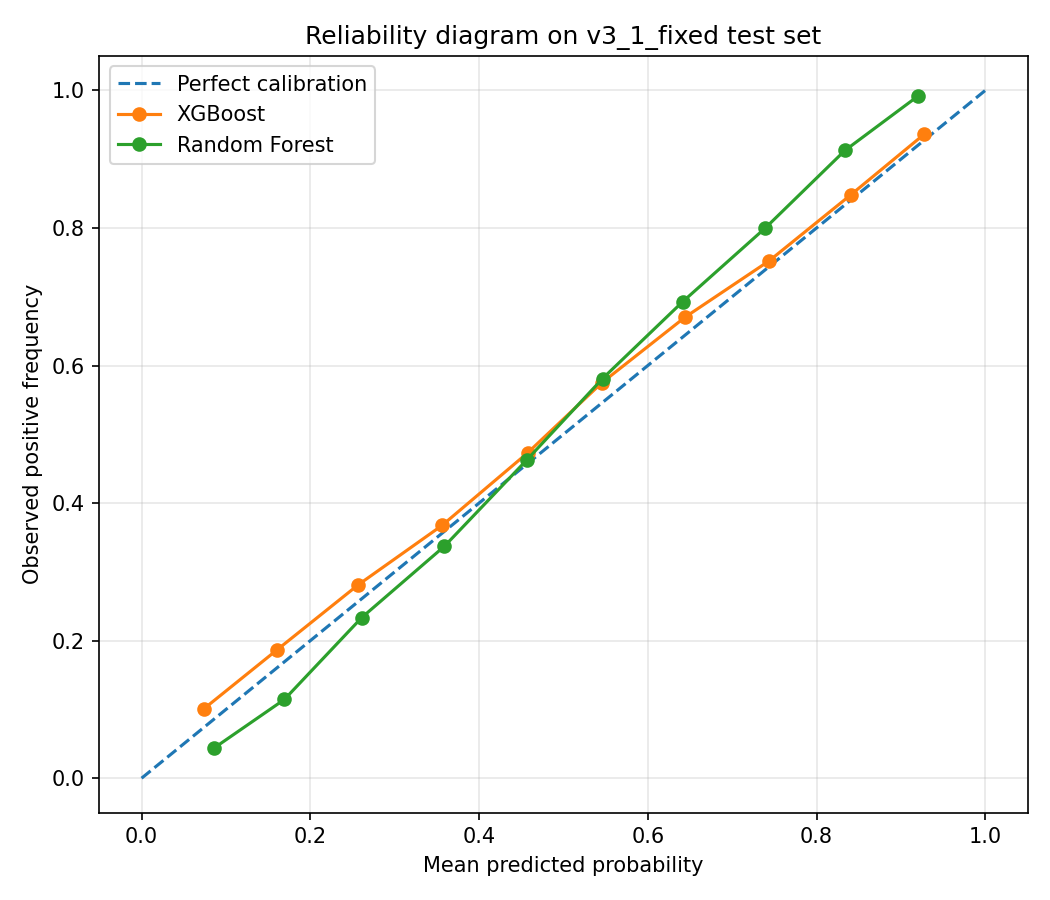
\includegraphics[width=0.74\textwidth]{../figures/test2_reliability_xgb_vs_rf.png}
    \caption{Reliability diagram for the frozen V3.1 fixed test split. XGBoost remains closer to the ideal calibration line across the probability bins, while Random Forest shows larger local deviations.}
\end{figure}

\subsection{Calibration completion with the final MLP export}
To close the probabilistic comparison across all final model families, the PyTorch MLP was re-exported on the same frozen \textbf{V3.1 fixed} test split and evaluated with the same 10-bin calibration protocol. The export run remained slightly below its earlier aligned benchmark but confirmed the same global ranking: XGBoost first, Random Forest second, and MLP third. Table~\ref{tab:calibration_xgb_rf_mlp} reports the final three-way calibration comparison.

\begin{table}[H]
\centering
\caption{Final three-way calibration comparison on the frozen V3.1 fixed test split. Lower Brier, log-loss, ECE, and MCE are better.}
\label{tab:calibration_xgb_rf_mlp}
\begin{tabularx}{\textwidth}{>{\raggedright\arraybackslash}p{2.8cm} >{\centering\arraybackslash}p{1.65cm} >{\centering\arraybackslash}p{1.65cm} >{\centering\arraybackslash}p{1.65cm} >{\centering\arraybackslash}p{1.65cm} >{\centering\arraybackslash}p{1.65cm}}
\toprule
Model & Brier & LogLoss & ROC-AUC & ECE & MCE \\
\midrule
XGBoost & \textbf{0.2273} & \textbf{0.6451} & \textbf{0.6665} & \textbf{0.0208} & \textbf{0.0294} \\
Random Forest & 0.2286 & 0.6483 & 0.6642 & 0.0294 & 0.0791 \\
MLP PyTorch & 0.2289 & 0.6488 & 0.6620 & 0.0328 & 0.0409 \\
\bottomrule
\end{tabularx}
\end{table}

The additional MLP calibration run does not change the decision logic of the paper; it strengthens it. XGBoost remains best on every reported calibration-related metric, Random Forest remains a very strong second model with weaker probability quality but nearly tied discrimination, and the MLP lags behind both tree ensembles. Interestingly, MLP shows lower MCE than Random Forest, suggesting fewer extreme local deviations, but it is still worse on Brier score, log-loss, ROC-AUC, and ECE. The overall probabilistic ordering therefore remains \emph{XGBoost $>$ Random Forest $>$ MLP}.

\begin{figure}[H]
    \centering
    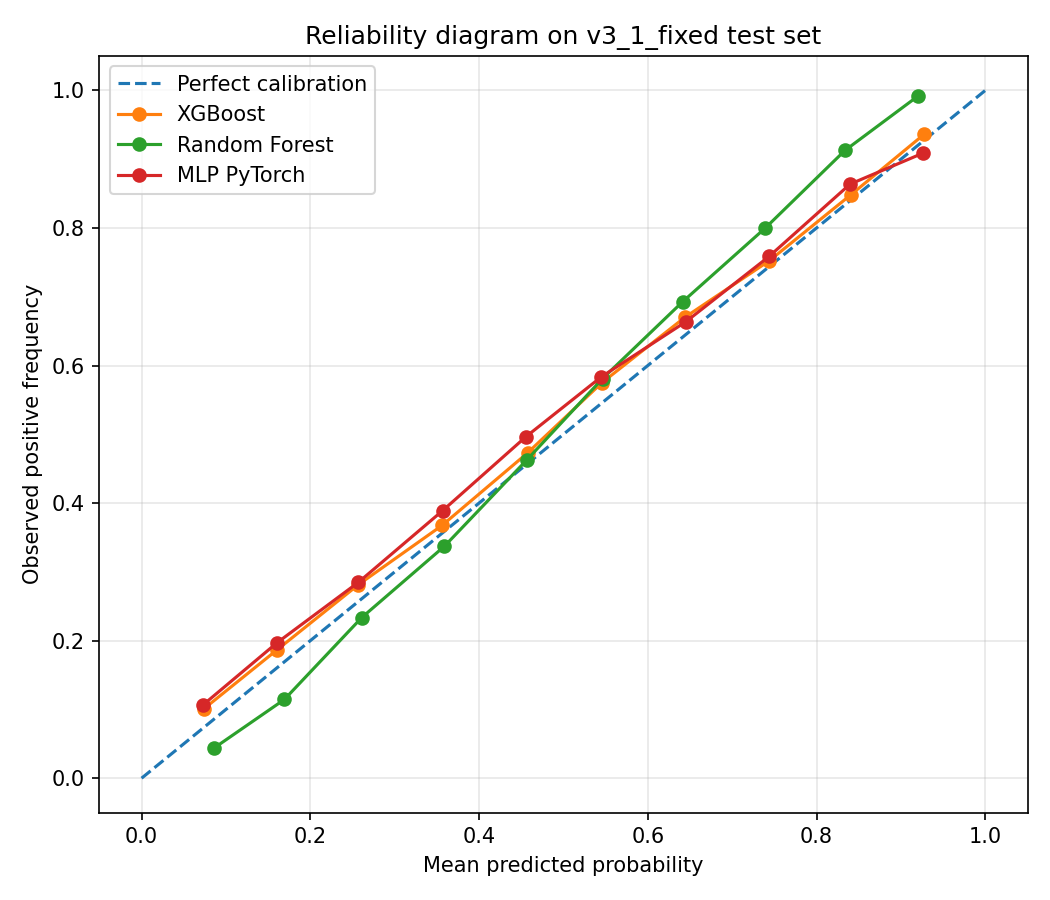
\includegraphics[width=0.74\textwidth]{../figures/test4_reliability_xgb_rf_mlp.png}
    \caption{Final three-way reliability diagram on the frozen V3.1 fixed test split. XGBoost remains closest to ideal calibration overall, Random Forest is highly competitive but shows larger local deviations, and MLP PyTorch is systematically less calibrated than the two tree ensembles.}
\end{figure}

\subsection{Older comparison table kept for historical context}
Table~\ref{tab:legacy_summary} records the earlier compact-project snapshot. It remains useful as historical context because it illustrates how misleading row-based validation can be.

\begin{table}[H]
\centering
\caption{Earlier project snapshot kept for historical context. ``Real'' refers to replay-aware validation; ``Falsified'' refers to row-based validation affected by leakage.}
\label{tab:legacy_summary}
\begin{tabularx}{\textwidth}{>{\raggedright\arraybackslash}p{2.7cm} >{\raggedright\arraybackslash}X >{\centering\arraybackslash}p{2.2cm} >{\centering\arraybackslash}p{2.4cm}}
\toprule
Model & Paradigm & Accuracy (real) & Accuracy (falsified) \\
\midrule
XGBoost & Gradient boosting (GPU) & 60.70\% & 87.34\% \\
Random Forest & Bagging trees & 60.85\% & 86.10\% \\
MLP & Deep feedforward network (GPU) & 60.34\% & 79.20\% \\
SVM & RBF margin model, reduced subset & 58.45\% & 68.19\% \\
\bottomrule
\end{tabularx}
\end{table}

\subsection{Frozen ablation and reproducibility table}
\begin{table}[H]
\centering
\caption{Frozen ablation summary under the uniform replay-aware XGBoost protocol. Every dataset contains 892,047 snapshots derived from 23,241 replays, split into 14,873 training replays, 3,719 validation replays, and 4,649 test replays.}
\label{tab:ablation_summary}
\begin{tabularx}{\textwidth}{>{\raggedright\arraybackslash}p{2.9cm} >{\centering\arraybackslash}p{1.2cm} >{\centering\arraybackslash}p{1.35cm} >{\centering\arraybackslash}p{1.25cm} >{\centering\arraybackslash}p{1.3cm} >{\centering\arraybackslash}p{1.3cm} >{\centering\arraybackslash}p{1.2cm} >{\centering\arraybackslash}p{1.3cm}}
\toprule
Dataset & Feat. & CV Acc. & Test Acc. & Bal. Acc. & ROC-AUC & LogLoss & Best iter. \\
\midrule
Baseline clean & 27 & 0.5955 & 0.6063 & 0.6016 & 0.6509 & 0.6529 & 257 \\
V2 dynamic & 55 & 0.6007 & 0.6158 & 0.6118 & 0.6618 & 0.6477 & 367 \\
V3.1 fixed & 64 & 0.6066 & 0.6193 & 0.6154 & \textbf{0.6665} & \textbf{0.6451} & 488 \\
V3.2 combatfix & 73 & \textbf{0.6019} & \textbf{0.6195} & \textbf{0.6155} & 0.6660 & 0.6454 & 601 \\
\bottomrule
\end{tabularx}
\end{table}


\section{Feature Importance and Interpretation}
The newer experiments sharpen the interpretation considerably. In the compact baseline, worker difference already dominated the feature ranking. After the parser revisions, the most stable and influential variables are now:
\begin{itemize}
    \item \texttt{diff\_income} and \texttt{diff\_workers},
    \item longer-horizon economic dynamics such as \texttt{diff\_income\_60s} and \texttt{diff\_income\_120s},
    \item combat-related summaries such as \texttt{diff\_combat\_score} or, in the combatfix branch, \texttt{diff\_raw\_army\_power},
    \item scouting signals and number-of-unit-types features,
    \item repaired tech variables such as \texttt{tech\_diff} and player-specific tech levels.
\end{itemize}

This evolution is scientifically important. It shows that the project has moved from a mostly macroeconomic predictor toward a more balanced representation that combines economy, temporal momentum, composition complexity, scouting, and technology timing. In particular, the jump from V2 to V3.1 confirms that the earlier constants/counters layer was not being exploited correctly: once its semantics were fixed, technology-related variables became genuinely useful.

\begin{figure}[H]
    \centering
    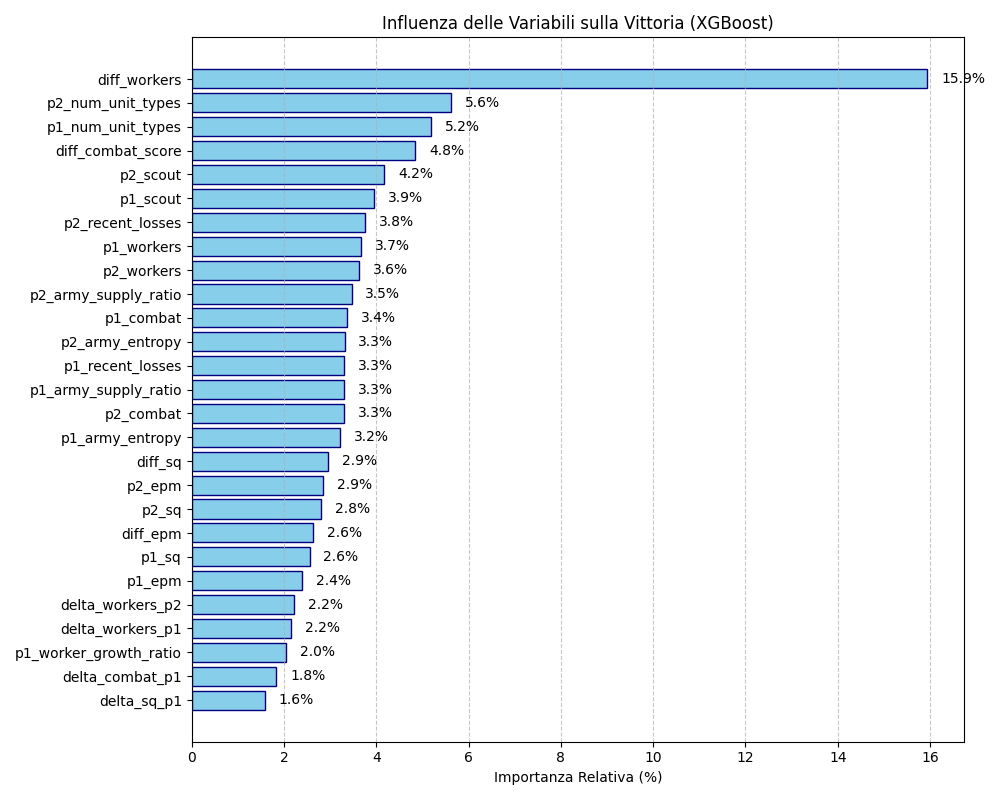
\includegraphics[width=0.83\textwidth]{../figures/feature_importance_baseline.png}
    \caption{Earlier XGBoost feature-importance visualization from the compact feature set. It is retained as a baseline reference.}
\end{figure}

\begin{figure}[H]
    \centering
    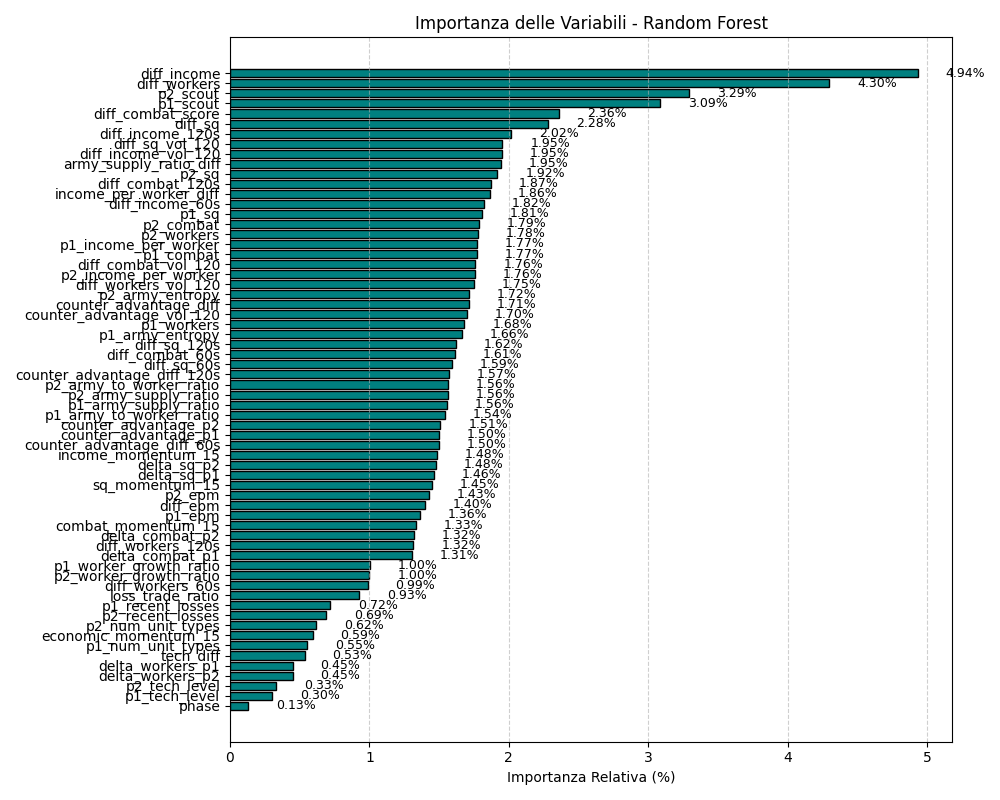
\includegraphics[width=0.90\textwidth]{../figures/rf_feature_importance_v3_1.png}
    \caption{Random Forest feature importance on the V3.1 fixed dataset. The ranking is broadly consistent with the improved XGBoost runs: economy and momentum dominate, while scouting, combat, and counter/tech-related features contribute additional signal.}
\end{figure}

\begin{figure}[H]
    \centering
    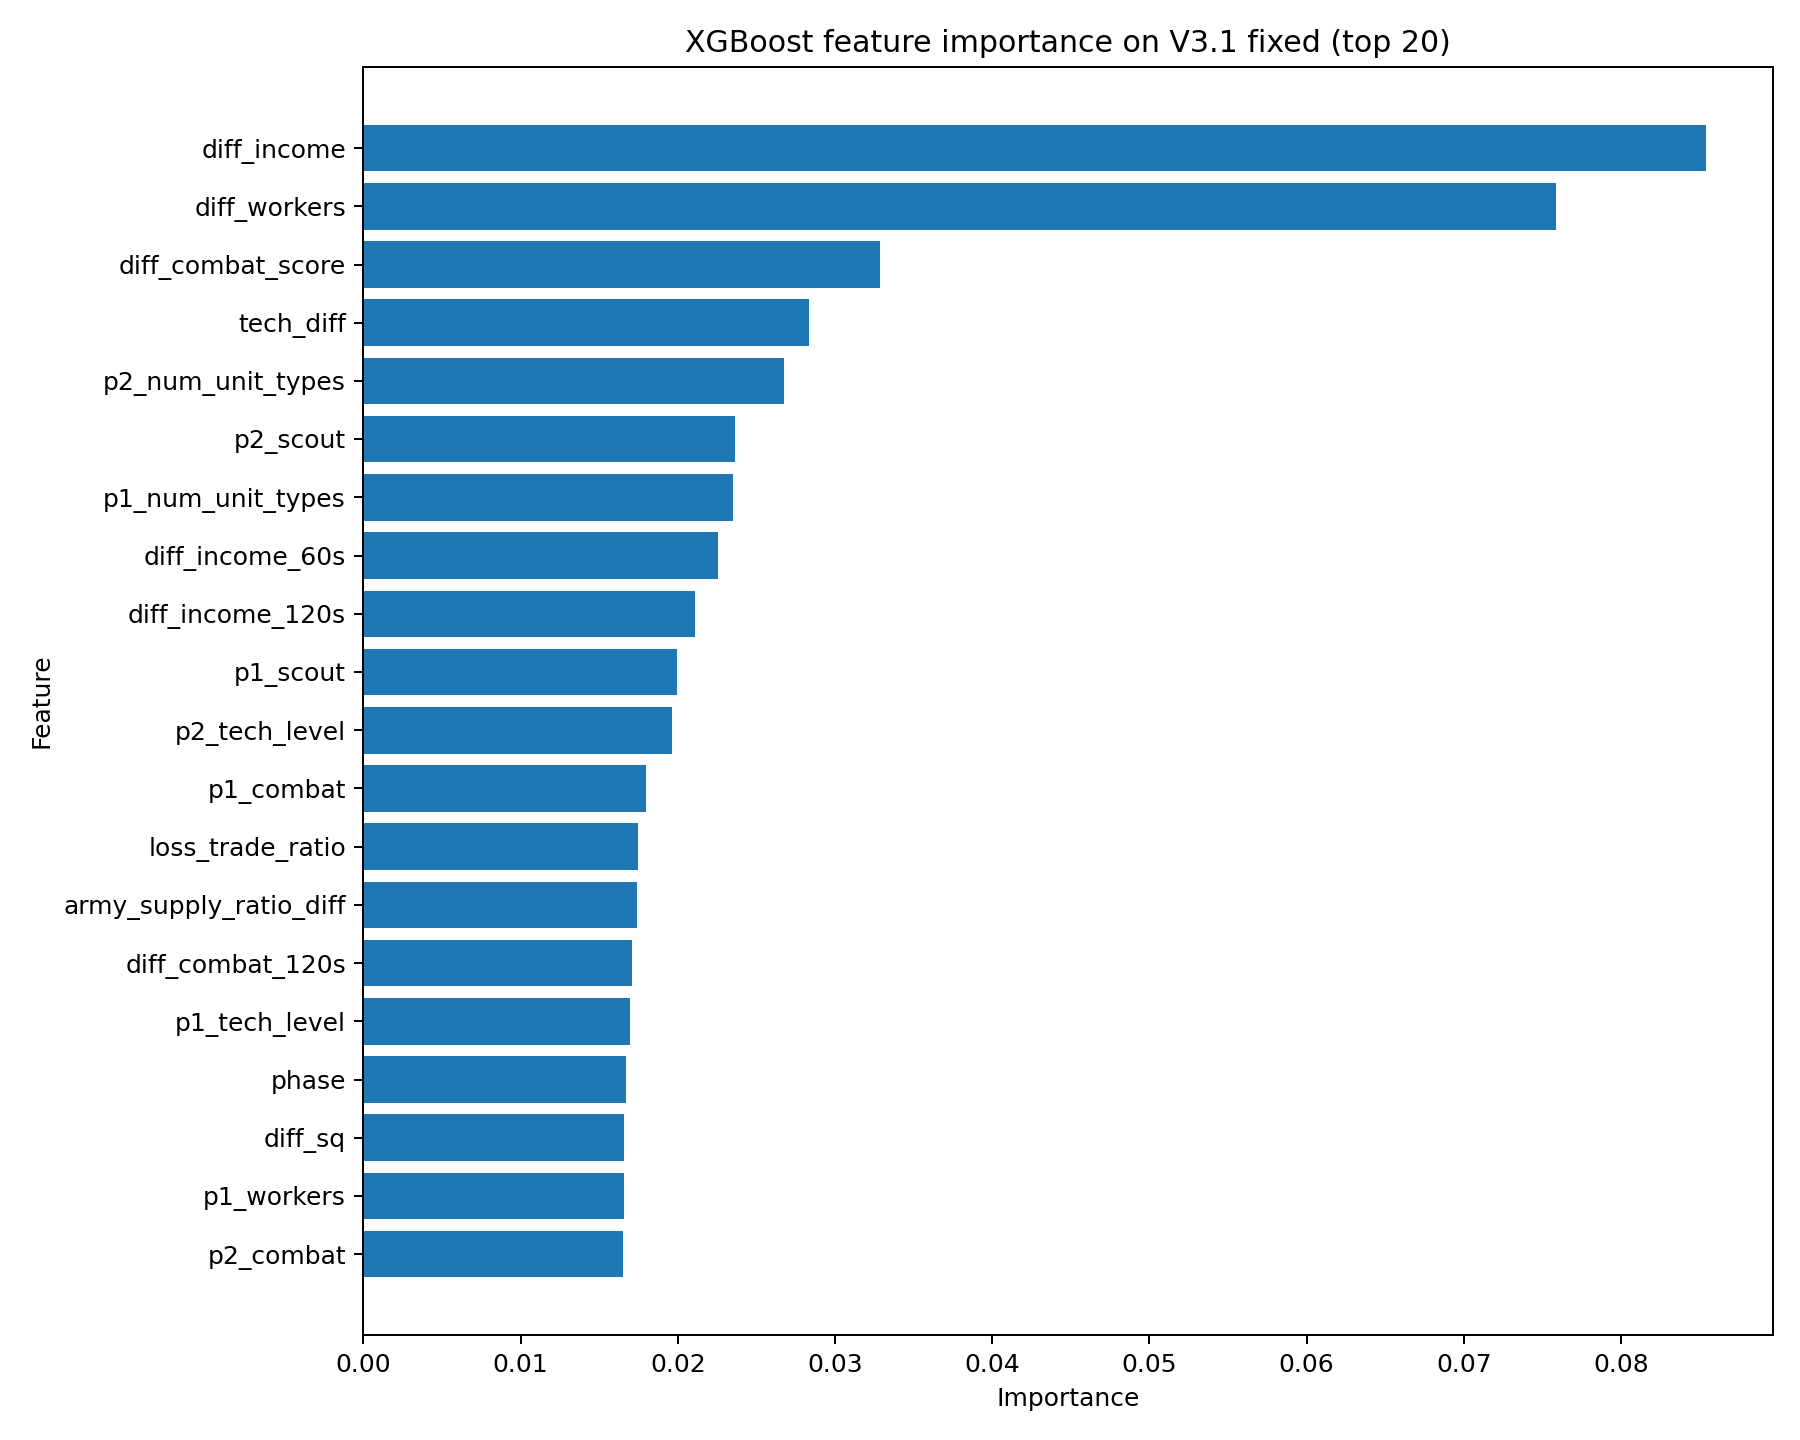
\includegraphics[width=0.88\textwidth]{../figures/xgb_feature_importance_v3_1_fixed.png}
    \caption{XGBoost feature importance on the frozen V3.1 fixed dataset. Economy and worker advantage remain dominant, while technology, combat, and army-complexity variables contribute the secondary signal that separates the richer parser branch from the earlier compact baseline.}
\end{figure}

\section{Temporal Analysis by Match Duration}
The unified duration comparison is now available for all three final models on the frozen \textbf{V3.1 fixed} test split. The comparison was built replay-aware: each snapshot inherits the total duration of its replay through the maximum observed \texttt{time\_sec} for that replay, and all models are then evaluated on the same duration bins with matched \texttt{n\_samples} and \texttt{n\_replays}. The resulting comparison confirms that the late-game weakness is a shared property of the representation rather than a model-family-specific failure mode.

Table~\ref{tab:duration_compare} summarizes the final duration-binned accuracy values. The strongest regime for all models remains the standard mid-game region around 5--10 minutes, where XGBoost is best overall. Random Forest is extremely competitive throughout and becomes slightly stronger than XGBoost in the longer bins. The PyTorch MLP remains consistently below both tree-based models in every populated bin.

\begin{table}[H]
\centering
\caption{Final unified duration comparison on the frozen V3.1 fixed test split. All three models use the same replay-derived duration bins.}
\label{tab:duration_compare}
\begin{tabular}{lccccc}
\toprule
Duration bin & XGBoost & Random Forest & MLP PyTorch & $n_{samples}$ & $n_{replays}$ \\
\midrule
0 min  & 0.5853 & 0.6153 & 0.5475 & 1,799  & 217 \\
5 min  & \textbf{0.6435} & 0.6360 & 0.6300 & 38,911 & 1,705 \\
10 min & \textbf{0.6285} & 0.6268 & 0.6227 & 69,353 & 1,719 \\
15 min & 0.6119 & \textbf{0.6144} & 0.6075 & 41,627 & 688 \\
20 min & 0.5770 & \textbf{0.5770} & 0.5691 & 19,627 & 246 \\
25 min & 0.5684 & \textbf{0.5820} & 0.5622 & 7,382  & 74 \\
\bottomrule
\end{tabular}
\end{table}

The important conclusion is not that one model dominates every duration regime, but that \emph{all} models lose accuracy in very long matches. The common decline after roughly 15--20 minutes suggests a representation ceiling: the current tabular state abstraction appears sufficient for economy, scouting, and medium-horizon momentum, but less sufficient for rich late-game composition, positioning, and hidden-information interactions.

\begin{figure}[H]
    \centering
    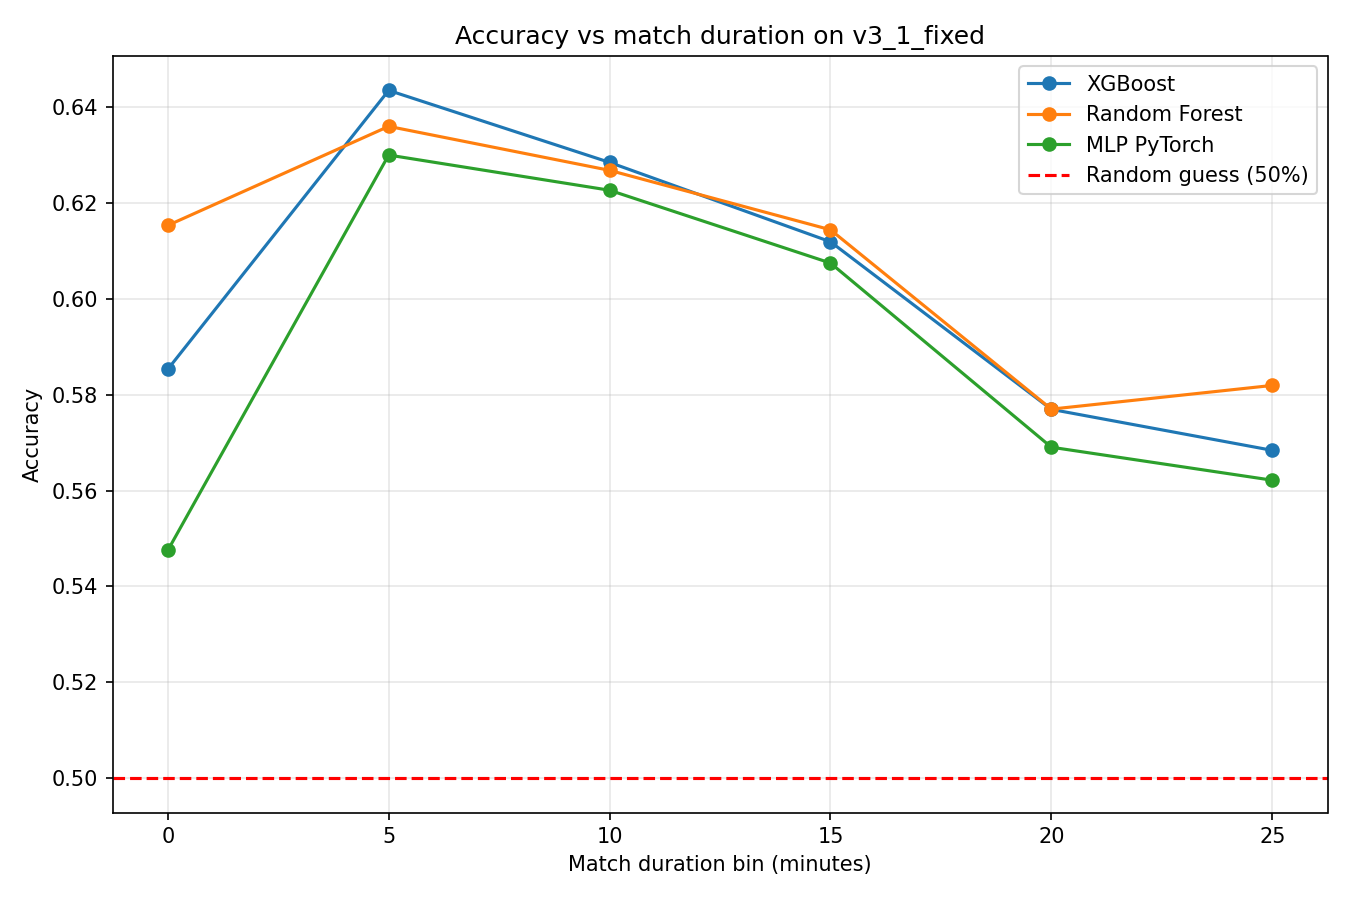
\includegraphics[width=0.82\textwidth]{../figures/test3_duration_comparison_v3_1.png}
    \caption{Final unified duration-based accuracy comparison on V3.1 fixed. XGBoost is strongest overall in the dominant 5--10 minute regime, Random Forest remains extremely close and can be slightly stronger in the longest bins, and MLP PyTorch stays consistently below both tree ensembles.}
\end{figure}

\begin{figure}[H]
    \centering
    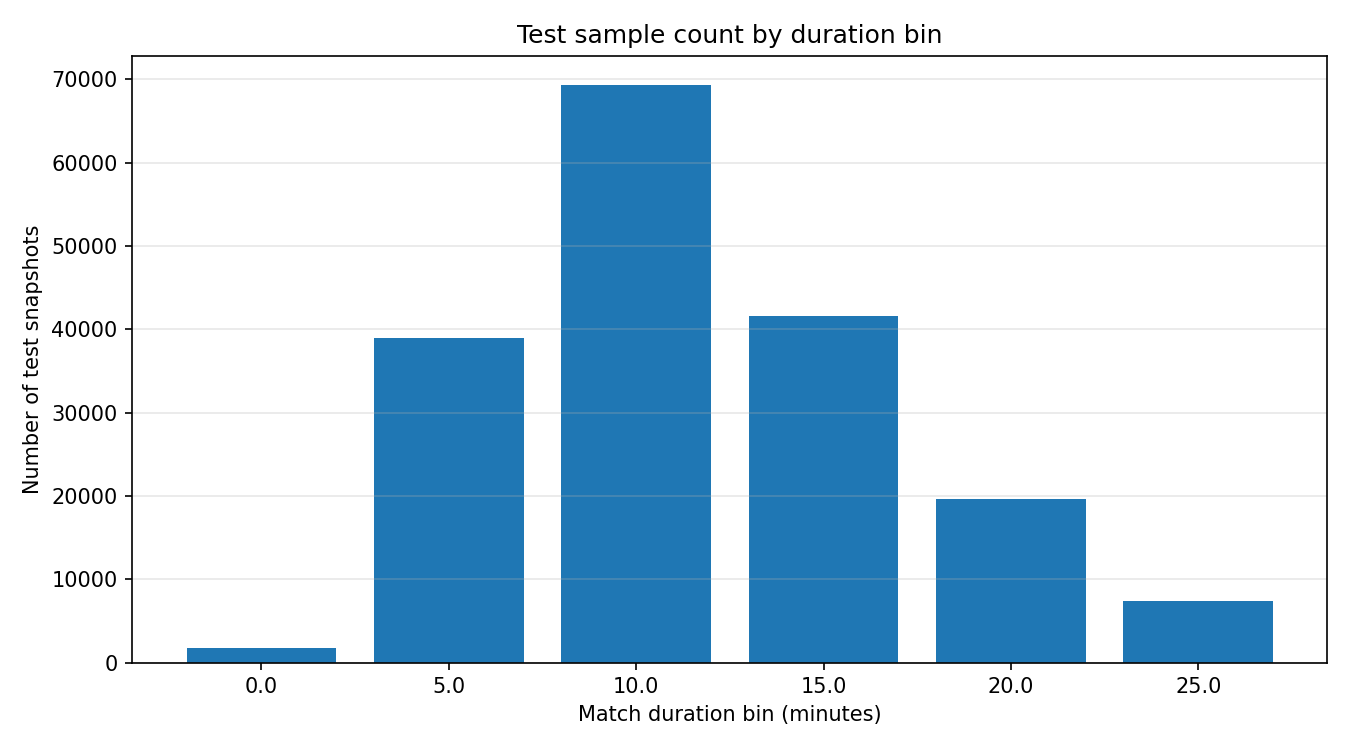
\includegraphics[width=0.74\textwidth]{../figures/test3_duration_comparison_v3_1_sample_counts.png}
    \caption{Test sample count by duration bin for the unified duration comparison. The longer-duration bins are noticeably smaller, which should be kept in mind when interpreting late-game differences.}
\end{figure}

\section{Critical Discussion}
\subsection{Why the absolute accuracy is not extremely high}
A 61\% replay-aware accuracy may appear modest at first glance, but it is actually plausible for this representation. The dataset deliberately compresses a complex partially observed game into periodic scalar summaries. This loses:
\begin{itemize}
    \item spatial positioning,
    \item engagement geometry,
    \item local terrain context,
    \item exact fog-of-war knowledge,
    \item fine-grained micro control.
\end{itemize}
Therefore, the model is predicting the winner from strategic summaries rather than from the full state of the game.

\subsection{What the models are probably learning}
The best interpretation is that the models learn \emph{strategic momentum} rather than tactical certainty. They can detect when one player has accumulated enough economic, scouting, and army-structure advantage that the match becomes more likely to end in their favor. They are much weaker when the eventual result depends on hidden information, one decisive engagement, or execution details invisible to the feature space.

\subsection{Why trees currently dominate}
The current results support the claim that tree ensembles are the safest default on this dataset. This does not mean deep learning is useless here. It means that with independent tabular snapshots and a relatively compact hand-engineered feature set, the inductive bias of trees may be more aligned with the problem than that of a feedforward neural network.

\section{Threats to Validity}
The current project should explicitly acknowledge the following validity threats:
\begin{enumerate}
    \item \textbf{Parser-feature mismatch across branches.} The codebase already contains richer parser versions than the feature set used in the first completed experiments.
    \item \textbf{Non-identical model-selection procedures across families.} XGBoost and Random Forest use grouped GridSearchCV, whereas the PyTorch MLP uses validation-based candidate selection over a smaller configuration set.
    \item \textbf{Potential instability in late-game bins.} Very long games may be underrepresented, causing noisy duration trends.
    \item \textbf{Representation ceiling.} Tabular snapshots may simply omit too much information for large gains without sequence or spatial modeling.
\end{enumerate}

\section{Roadmap for the Final Paper Cycle}
The benchmark phase is now sufficiently closed that the remaining work should emphasize \emph{artifact freezing, editorial consolidation, and optional polish} rather than new parser branches. The recommended order is:

\begin{enumerate}
    \item \textbf{Freeze the benchmark artifacts.} Keep \textbf{V3.1 fixed} as the principal reported dataset branch, retain \textbf{V3.2 combatfix} as the combat-representation ablation, and archive the final logs, summaries, prediction files, bootstrap outputs, calibration outputs, and paper sources.
    \item \textbf{Finalize the interpretation section.} The paper should now explicitly state that feature engineering and parser semantics account for the largest gains, while the algorithmic margin between the two strongest tree ensembles is small on accuracy but meaningful on probabilistic quality.
    \item \textbf{Polish the final presentation.} Tighten naming consistency, remove reserved writing placeholders that are no longer needed, and ensure the figures/tables referenced in the conclusions are the exact frozen ones.
    \item \textbf{Only then decide whether any new parser branch is justified.} A new V4 should be considered only if the remaining failure mode is clearly identified and if extending the project is preferable to freezing the final deliverable.
\end{enumerate}

\section{Final Freeze Checklist and Remaining Editorial Tasks}
This section records the final freeze status after closing the main benchmark, the replay-bootstrap significance test, the tree-ensemble calibration comparison, the unified duration comparison, and the optional MLP calibration completion.

\begin{longtable}{>{\raggedright\arraybackslash}p{3.2cm} >{\raggedright\arraybackslash}p{8.4cm} >{\raggedright\arraybackslash}p{3.1cm}}
\caption{Freeze checklist and remaining editorial work after closing the benchmark, replay-bootstrap test, calibration analysis, duration comparison, and optional MLP calibration completion.}\\
\toprule
Item & What must be done & Priority \\
\midrule
\endfirsthead
\toprule
Item & What must be done & Priority \\
\midrule
\endhead
Unified duration comparison & \textbf{Completed.} Final replay-aware duration table and figures have been generated for XGBoost, Random Forest, and MLP on the frozen V3.1 split. & Closed \\
Optional calibration of MLP & \textbf{Completed.} MLP probabilities were exported on the frozen split and incorporated into the final three-way calibration comparison. & Closed \\
Final artifact freeze & Archive the exact final dataset version, summary JSON files, prediction CSV files, bootstrap outputs, calibration outputs, execution logs, and paper sources used to produce the final tables. & High \\
Cross-model discussion polish & Tighten the explanation of why XGBoost is selected as the main model despite the replay-bootstrap showing no strong 95\% superiority over Random Forest on accuracy and AUC. & Medium \\
Optional V4 decision & Decide whether any new parser branch is justified only after artifact freezing and final editorial cleanup are complete. & Low \\
\bottomrule
\end{longtable}

\subsection*{Methodology of the remaining finalization work}
Only a small amount of methodological work remains.
\begin{itemize}
    \item \textbf{Artifact freeze methodology.} Preserve the exact scripts, prediction exports, summary JSON files, bootstrap outputs, calibration outputs, execution logs, and paper sources corresponding to the final paper tables. Do not silently replace them with later reruns under different naming conventions.
    \item \textbf{Editorial consistency methodology.} Keep version naming fixed across all text, tables, and manifests: \texttt{baseline\_clean}, \texttt{v2\_dynamic}, \texttt{v3\_1\_fixed}, and \texttt{v3\_2\_combatfix}. Keep \texttt{V3.1 fixed} as the principal benchmark branch.
    \item \textbf{Optional extension methodology.} Any further V4 parser work should be explicitly labeled as a post-freeze extension and should not overwrite the frozen artifacts reported in this paper.
\end{itemize}

\section{Conclusion}
At its current stage, the project already supports a strong technical narrative. It demonstrates that match prediction in StarCraft II from tabular replay snapshots is feasible, but only if the pipeline is treated as a full machine learning system rather than a simple classifier benchmark. The main methodological contribution is the elimination of replay leakage through grouped evaluation. The main empirical result is that once validation is corrected and the parser is improved, the strongest baselines converge near 62\% accuracy, with the dominant gains coming from better feature semantics and temporal representation rather than from changing the learning algorithm alone.

The final cross-model comparison sharpens that claim. XGBoost is the best overall model on the frozen V3.1 dataset, Random Forest is almost tied across the main metrics, and the GPU-trained PyTorch MLP remains consistently below the two tree ensembles. The paired replay-bootstrap refines the interpretation: XGBoost does not show a statistically strong 95\% advantage over Random Forest on accuracy or ROC-AUC, but it does show a statistically supported advantage in log-loss. The calibration analysis then strengthens that conclusion further. In the two-model tree comparison, XGBoost is better calibrated than Random Forest, with lower Brier score, lower ECE, and much lower MCE on the frozen test split. The optional three-way calibration completion preserves the same ordering: XGBoost remains best on all reported probability-quality metrics, Random Forest remains second, and MLP is third overall despite having a lower MCE than Random Forest. This is a good outcome, not a disappointing one. It means the project has already moved past naive benchmark inflation and reached the stage where progress must come from better representation, cleaner experiments, and more explicit temporal and counter-based modeling. In other words, the main reason to prefer XGBoost is no longer a large gain in raw accuracy, but the combination of near-best discrimination and clearly better probabilistic quality.

\section{Conceptual Extension: A POMDP-like View of Replay Snapshots}
Although the present study is framed as a supervised learning problem over tabular replay snapshots, the underlying \emph{StarCraft II} process is naturally partially observable. The true strategic state of a match at time $t$ is richer than the compact feature vector exposed to the predictive models. It includes latent or only partially visible factors such as hidden tech choices, spatial pressure, future production intent, local tactical geometry, and information asymmetry. For this reason, the current pipeline also admits a useful \emph{POMDP-like} conceptual interpretation.

Let $s_t \in S$ denote the latent strategic state of the match at time $t$, and let $o_t \in O$ denote the observed replay snapshot extracted by the parser and feature engineering pipeline. Under this view, the dataset does not provide direct access to the full strategic state. Instead, it provides a compact and engineered observation of that state, built from economy, army composition, scouting, recent losses, and short-horizon temporal deltas. A high-level action space $A$ can then be introduced conceptually, where actions correspond not to low-level game commands but to abstract strategic choices such as economic investment, worker growth, military production, defensive stabilization, offensive pressure, or additional scouting.

In this interpretation, match evolution may be described by a transition model $T(s_{t+1}\mid s_t, a_t)$ and an observation model $Z(o_{t+1}\mid s_{t+1}, a_t)$, where the quality of the future observation is influenced by partial information and scouting quality. Historical replay trajectories can then be viewed as empirical evidence for estimating a belief-like representation over latent strategic situations. The current project does not explicitly solve a POMDP, perform belief updates, or optimize a sequential policy. However, the replay dataset can still be interpreted as a collection of observation sequences that act as proxies for hidden strategic states and that could support future work on latent-state estimation, action valuation, or policy recommendation under partial observability.

This perspective should be understood as a conceptual extension rather than a redefinition of the present contribution. The main result of the paper remains a rigorous replay-aware machine learning pipeline for match outcome prediction. Nevertheless, the POMDP-like view is useful because it clarifies why static tabular snapshots already contain meaningful strategic signal while also explaining why future progress may require richer temporal modeling, belief-like state tracking, and more explicit reasoning over strategic actions. For a compact standalone formal note corresponding to this interpretation, the freeze package includes \texttt{paper/appendix\_reference\_sc2\_pomdp\_like\_spec.pdf}.

\appendix
\section{Appendix A: Snapshot of the Current Code Logic}
The project files currently indicate the following status:
\begin{itemize}
    \item a baseline parser and bridge used for the earlier compact dataset,
    \item updated parser and bridge branches with explicit counter, momentum, volatility, tech-fix, and combat-refactor features,
    \item a stronger XGBoost script with proper outer split, inner split, grouped model selection, and early stopping,
    \item a stronger Random Forest script with grouped model selection,
    \item a GPU-aware PyTorch MLP script using replay-aware train/validation/test splitting and validation-based candidate selection.
\end{itemize}

\section{Appendix B: Final Freeze Manifest}
The final freeze package archives the exact paper sources, benchmark summaries, prediction exports, bootstrap outputs, calibration outputs, methodology notes, and execution logs used in the closing experimental cycle. The frozen benchmark logic is therefore:
\begin{itemize}
    \item principal dataset branch: \textbf{V3.1 fixed},
    \item principal model: \textbf{XGBoost},
    \item strongest alternative baseline: \textbf{Random Forest},
    \item neural comparison model: \textbf{PyTorch MLP},
    \item parser-ablation branch retained for interpretation: \textbf{V3.2 combatfix}.
\end{itemize}
Any future V4 branch should be treated as a separate post-freeze extension rather than a silent replacement of these artifacts.

\section{Appendix C: Supplementary Reference Note for the POMDP-like View}
The final freeze package includes a short standalone note that expands the conceptual formulation introduced near the end of the main paper. This supplementary file is intended as an external appendix reference rather than as a new experimental claim. Its purpose is to formalize the distinction between latent strategic state, replay-derived observation, high-level strategic action, observation quality, and belief-like estimation from historical replay trajectories.

The supplementary reference note is archived as:
\begin{itemize}
    \item \texttt{paper/appendix\_reference\_sc2\_pomdp\_like\_spec.tex}
    \item \texttt{paper/appendix\_reference\_sc2\_pomdp\_like\_spec.pdf}
\end{itemize}

This material should be read as a conceptual extension and as a possible future theoretical direction. It does not change the empirical scope of the present study, which remains centered on replay-aware supervised outcome prediction.


\end{document}
